Այս պարագրաֆում կամփոփենք լրիվ բազմակողմանի գրաֆների միջակայքային ներկումների վերաբերյալ կատարված աշխատանքները և կապացուցենք մի շարք նոր արդյունքներ: Լրիվ բազմակողմանի գրաֆներից առաջինը ուսումնասիրվել են լրիվ երկկողմանի գրաֆները: Քամալյանին հաջողվել է լիարժեք պատասխանել այն հարցին, թե երբ և որքան գույներով միջակայքային ներկումներ կարող են ունենալ լրիվ երկկողմանի գրաֆները \cite{Kamalian1989}:

\begin{theorem}
\label{t1_complete_bipartite}
$K_{m,n}$ լրիվ երկկողմանի գրաֆը ունի միջակայքային $t$-ներկում այն և միայն դեպքում, երբ $m+n-(m,n) \leq t \leq m+n-1$:
\end{theorem}

Պետրոսյանը \cite{Petrosyan2012}-ում ստացել է որոշ արդյունքներ հավասարակշռված լրիվ բազմակողմանի գրաֆների համար, երբ գրաֆի բոլոր կողմերում գագաթների թիվը նույնն է:
\begin{theorem}
\label{t1-complete-balanced-Petrosyan}
Եթե $K_{n,\ldots,n}$ լրիվ հավասարակշռված $r$-կողմանի գրաֆ է, ապա
$K_{n,\ldots,n} \in \mathfrak{N}$ այն և միայն այն դեպքում, երբ $nr$-ը զույգ է: Ավելին, երբ $nr$-ը զույգ է, ապա $w(K_{n,\ldots,n}) = n(r-1)$ և $W(K_{n,\ldots,n}) \geq \left(
\frac{3}{2}r-1 \right)n-1$:
\end{theorem}

Եվս մեկ արդյունք ստացվել է Ֆենգի և Հուանգի կողմից \cite{FengHuang2007} լրիվ երեք կողմանի գրաֆների մի ենթադասի համար:
\begin{theorem}
\label{FengHuang}
Ցանկացած $n\in\mathbb{N}$ թվի համար, $K_{1,1,n}\in \mathfrak{N}$ այն և միայն դեպքում, երբ $n$-ը զույգ է:
\end{theorem}

Պետրոսյանը ``Cycles and Colorings 2012'' գիտաժողովում առաջարկել էր վերոհիշյալ թեորեմը ընդհանրացնող հետևյալ հիպոթեզը.
\begin{hypothesis}
Ցանկացած $m,n\in\mathbb{N}$ թվերի համար, $K_{1,m,n}\in\mathfrak{N}$ այն և միայն դեպքում, երբ
$(m+1,n+1)=1$:
\end{hypothesis}

Այս պարագրաֆում կապացուցենք այս հիպոթեզը, կստանանք մի շարք նոր արդյունքներ լրիվ երեք կողմանի գրաֆների այլ ենթադասերի համար և կլավացնենք Թեորեմ \ref{t1-complete-balanced-Petrosyan}-ի գնահատականը:

Նախ, ապացուցենք մի օժանդակ լեմմա լրիվ բազմակողմանի գրաֆների ընդհանուր դեպքի համար:
\begin{lemma}
\label{l1-k-partite-scale}
Եթե $K_{n_1,\dots,n_r} \in \mathfrak{N}$, ապա կամայական $d \in \mathbb{N}$ թվի համար $K_{dn_1, \ldots, dn_r} \in \mathfrak{N}$, ընդ որում $w(K_{dn_1, \ldots, dn_r}) \leq d \cdot w(K_{n_1, \ldots, n_r})$ և $W(K_{dn_1, \ldots, dn_k}) \geq d \cdot W(K_{n_1, \ldots, n_r}) + d - 1$:
\end{lemma}
\begin{proof}[Ապացույց]
$K_{dn_1, \ldots, dn_r}$ գրաֆը կարելի է ստանալ $K_{n_1, \ldots, n_r}$ գրաֆից յուրաքանչյուր գագաթի փոխարեն տեղադրելով $d$ գագաթներ և յուրաքանչյուր կող փոխարինելով $K_{d,d}$ լրիվ երկկողմանի գրաֆի կողերով համապատասխան գագաթների $d$-յակների միջև: Դիցուք,
\begin{align*}
    V(K_{n_1, \ldots, n_r}) &= \left\{u_i^j : j=1,\ldots,r,\ i=1,\ldots,n_j \right\}, \\
    V(K_{dn_1, \ldots, dn_r}) &= \left\{v_{i,s}^j : j=1,\ldots,r,\ i=1,\ldots,n_j,\ s=1,\ldots,d \right\}, \\
    V(K_{d,d}) &= \left\{x_s,y_s : s=1,\ldots,d\right\}:
\end{align*}
Դիցուք $\alpha$-ն $K_{n_1, \ldots, n_r}$ գրաֆի որևէ միջակայքային $t_{\alpha}$ ներկում է, իսկ $\beta$-ն $K_{d,d}$-ի որևէ սիմետրիկ միջակայքային $t_{\beta}$-ներկում, այսինքն $\beta(x_sy_{s'})=\beta(x_{s'}y_{s})$ կամայական $1 \leq s, s' \leq d$ թվերի համար: Կառուցենք $K_{dn_1, \ldots, dn_r}$-ի $\gamma$ կողային ներկումը հետևյալ կերպ.
\begin{align}
    \gamma(v_{i_1,s_1}^{j_1}v_{i_2,s_2}^{j_2}) &= r(\alpha(u_{i_1}^{j_1}u_{i_2}^{j_2})-1) + \beta(x_{s_1}y_{s_2}) \text{, որտեղ }\\
    &1 \leq j_1 \ne j_2 \leq r,\ 1\leq i_1 \leq n_{j_1},\ 1 \leq i_2 \leq n_{j_2},\ 1\leq s_1, s_2 \leq d:
\end{align}

Որպեսզի ցույց տանք, որ կառուցված ներկումը միջակայքային կողային ներկում է, հաշվենք գագաթների սպեկտրները: Կամայական $1 \leq j_1 \leq r$, $1\leq i_1 \leq n_{j_1}$ և $1\leq s_1 \leq d$ թվերի համար ունենք.
\begin{align*}
    S\left(v_{i_1,s_1}^{j_1}, \gamma\right) &= \bigcup\limits_{\substack{u_{i_2}^{j_2} \in V(K_{n_1, \ldots, n_r})\\ u_{i_1}^{j_1}u_{i_2}^{j_2} \in E(K_{n_1, \ldots, n_r})}}{
        \bigcup\limits_{s_2=1}^{d}{
            \gamma\left(v_{i_1,s_1}^{j_1}v_{i_2,s_2}^{j_2}\right)
        }
    }\\
    &= \bigcup\limits_{\substack{u_{i_2}^{j_2} \in V(K_{n_1, \ldots, n_r})\\ u_{i_1}^{j_1}u_{i_2}^{j_2} \in E(K_{n_1, \ldots, n_r})}}{
        \left[r(\alpha(u_{i_1}^{j_1}u_{i_2}^{j_2})-1) + \underline{S}(x_{s_1}, \beta), d(\alpha(u_{i_1}^{j_1}u_{i_2}^{j_2})-1) + \overline{S}(x_{s_1}, \beta) \right]
    }\\
    &= \left[d(\underline{S}(u_{i_1}^{j_1}, \alpha)-1) + \underline{S}(x_{s_1}, \beta), d(\overline{S}(u_{i_1}^{j_1},\alpha)-1) + \overline{S}(x_{s_1}, \beta) \right]:
\end{align*}
Դիցուք $K_{n_1, \ldots, n_r}$ գրաֆում $1$ և $t_{\alpha}$ գույները հասանելի են համապատասխանաբար $u_{i'}^{j'}$ և $u_{i''}^{j''}$ գագաթների վրա, իսկ $K_{d,d}$ գրաֆում $1$ և $t_{\beta}$ գույները հասանելի են համապատասխանաբար $x_{s'}$ և $x_{s''}$ գագաթների վրա: Այդ դեպքում $1 \in S\left(v_{i',s'}^{j'}, \gamma\right)$ և $dt_{\alpha}+t_{\beta}-d \in S\left(v_{i'',s''}^{j''}, \gamma\right)$: Ստացված արդյունքը ճիշտ է կամայական $\alpha$ և $\beta$ ներկումների համար: Ուստի, եթե որպես $\alpha$ վերցնենք $K_{n_1, \ldots, n_r}$-ի որևէ միջակայքային $W(K_{n_1, \ldots, n_r})$-ներկում, իսկ որպես $\beta$ վերցնենք $K_{d,d}$-ի միջակայքային $(2d-1)$-ներկումը (օրինակ՝ $\beta(x_s,y_t)=s+t-1$ բանաձևով տրվող), ապա կստանանք, որ $W(K_{dn_1, \ldots, dn_r}) \geq d\cdot W(K_{n_1, \ldots, n_r}) + d-1$: Իսկ եթե որպես $\alpha$ վերցնենք $K_{n_1, \ldots, n_r}$-ի որևէ միջակայքային $w(K_{n_1, \ldots, n_r})$-ներկում, իսկ որպես $\beta$ վերցնենք $K_{d,d}$-ի որևէ միջակայքային $d$-ներկում, ապա կստանանք, որ $w(K_{dn_1, \ldots, dn_r}) \leq d\cdot w(K_{n_1, \ldots, n_r})$:
\end{proof}

Այժմ անցնենք լրիվ երեք կողմանի գրաֆների քննարկմանը:

$K_{m,n}$ երկկողմանի գրաֆի երկու կողմերը նշանակենք $(U, V)$-ով, որտեղ $U = \left\{ u_0, u_1,
\ldots, u_{m-1} \right\}$ և $V = \left\{ v_0, v_1, \ldots, v_{n-1} \right\}$:
$K_{m,n}$-ի $\alpha_{m,n}$ միջակայքային կողային ներկումը մաքսիմալ թվով գույներով ներկումը տրվում է հետևյալ կերպ \cite{Kamalian1989}.
\begin{center}
$ \alpha_{m,n}(u_iv_j) = i+j+1$, որտեղ
$0 \leq i \leq m-1$, \hspace{3pt} $0 \leq j \leq n-1$:
\end{center}
$K_{1,m,n}$-ը լրիվ երեք կողմանի գրաֆ է, որը կարելի է դիտարկել որպես $K_{m,n}$ և նրան ավելացված մեկ նոր գագաթ, որը միացած է մյուս բոլոր գագաթներին: Այս հոդվածում մենք կապացուցենք, որ եթե $m+1$ և $n+1$ թվերը փոխադարձաբար պարզ են, ապա հնարավոր է $K_{m,n}$-ի $\alpha_{m,n}$ ներկումը լրացնել մինչև 
$K_{1,m,n}$-ի միջակայքային ներկում: Այնուհետև մենք կապացուցենք, որ եթե $(m+1,n+1) > 1$, ապա $K_{1,m,n}$-ը միջակայքային ներկելի չէ:

\begin{figure}
\centering
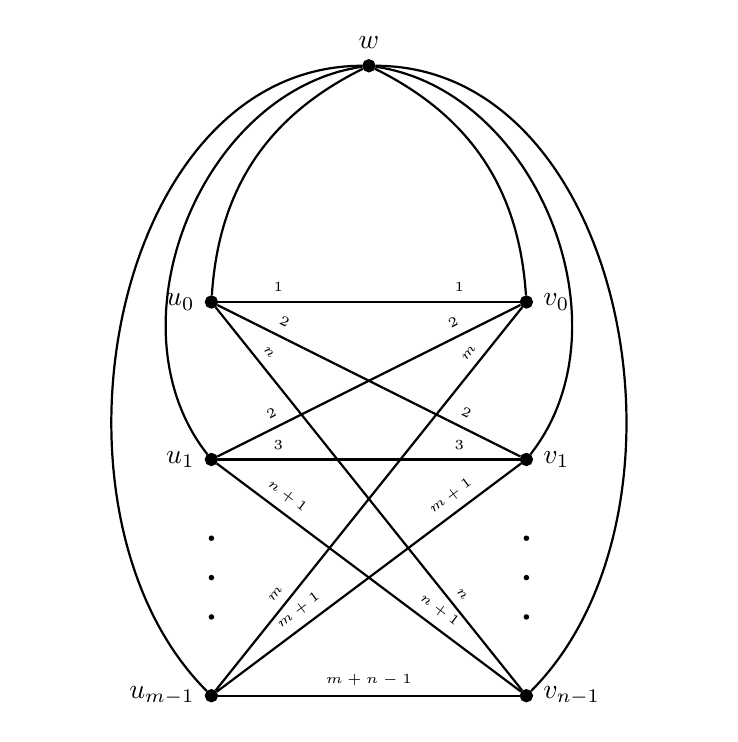
\begin{tikzpicture}
[thick,vertex/.style={circle,inner sep=0pt,minimum size=4pt,draw,fill=black}]
\node[vertex, label={right:$v_{n-1}$}] (vn) at ( 2,1) {} ;
\node[vertex, label={right:$v_{1}$}] (v1) at ( 2,4) {};
\node[vertex, label={right:$v_{0}$}] (v0) at ( 2,6) {};
\node[vertex, label={left:$u_{m-1}$}] (um) at (-2,1) {}
  edge node[sloped,above,pos=0.23] {\tiny $m$} node[sloped,above,pos=0.86] {\tiny $m$} (v0)
  edge node[sloped,above,pos=0.3] {\tiny $m+1$} node[sloped,above,pos=0.8] {\tiny $m+1$} (v1)
  edge node[auto] {\tiny $m+n-1$} (vn);
  
\node[vertex, label={left:$u_{1}$}] (u1) at (-2,4) {}
  edge node[sloped,above,pos=0.2] {\tiny $2$} node[sloped,above,pos=0.8] {\tiny $2$} (v0)
  edge node[sloped,above,pos=0.2] {\tiny $3$} node[sloped,above,pos=0.8] {\tiny $3$} (v1)
  edge node[sloped,above,pos=0.2] {\tiny $n+1$} node[sloped,above,pos=0.7] {\tiny $n+1$} (vn);
  
\node[vertex, label={left:$u_{0}$}] (u0) at (-2,6) {}
  edge node[sloped,above,pos=0.2] {\tiny $1$} node[sloped,above,pos=0.8] {\tiny $1$} (v0)
  edge node[sloped,above,pos=0.2] {\tiny $2$} node[sloped,above,pos=0.8] {\tiny $2$} (v1)
  edge node[sloped,above,pos=0.14] {\tiny $n$} node[sloped,above,pos=0.77] {\tiny $n$} (vn);
\node[vertex, label={above:$w$}] (w)  at ( 0,9) {}
  edge [bend right] (u0)
  edge [bend right=60] (u1)
  edge [out=180, in=135] (um)
  edge [bend left] (v0)
  edge [bend left=60] (v1)
  edge [out=0, in=45] (vn);
\fill (-2,2) circle (1pt);
\fill (-2,2.5) circle (1pt);
\fill (-2,3) circle (1pt);
\fill (2,2) circle (1pt);
\fill (2,2.5) circle (1pt);
\fill (2,3) circle (1pt);
\end{tikzpicture}

\caption{$K_{1,m,n}$ գրաֆը և $\alpha_{m,n}$ ներկումը}
\label{graphK1mn}
\end{figure}

$\alpha_{m,n}$ ներկման ժամանակ գագաթների սպեկտրները հետևյալն են.
\begin{center}
\begin{tabular}{cc}
$ S(u_i, \alpha_{m,n}) = [i+1, i+n ]$, & $0 \leq i \leq m-1$ \\
$ S(v_j, \alpha_{m,n}) = [j+1, j+m ]$, & $0 \leq j \leq n-1$
\end{tabular}
\end{center}

$K_{1,m,n}$ գրաֆը ստանանք $K_{m,n}$-ին ավելացնելով $w$ նոր գագաթը և միացնելով այն բոլոր մյուս գագաթների հետ:
\begin{align*}
V(K_{1,m,n}) & = V(K_{m,n}) \cup \{w\} \\
E(K_{1,m,n}) & = E(K_{m,n}) \cup \{u_iw : 0 \leq i \leq m-1 \} \cup \{v_jw : 0 \leq j \leq n-1 \}
\end{align*}

\begin{figure}[t]
\centering
\includegraphics[width=\textwidth]{figures/tripartite_auxillary.pdf}
\caption{Թեորեմ \ref{t1_K1mn_coprime}-ում կառուցված $H$ օժանդակ գրաֆը}
\label{graphH}
\end{figure}

\begin{theorem}
\label{t1_K1mn_coprime}
Եթե $(m+1,n+1)=1$, ապա $K_{1,m,n}$-ը ունի միջակայքային $(m+n)$-ներկում:
\end{theorem}
\begin{proof}[Ապացույց]
$K_{1,m,n}$-ի $u_iv_j$ կողերը ներկենք ճիշտ այնպես, ինչպես $\alpha_{m,n}$-ում: Թեորեմն ապացուցելու համար բավարար է ցույց տալ, որ մնացած կողերը հնարավոր է ներկել այնպես, որ բավարարվեն հետևյալ պահանջները.
\begin{description}
\item[(1)] $u_i$ և $v_j$ գագաթների սպեկտրները մնան ամբողջ թվերի միջակայքեր
\item[(2)] $w$ գագաթի սպեկտրը ևս լինի ամբողջ թվերի միջակայք
\end{description}
Կառուցենք օժանդակ $H$ երկկողմանի գրաֆը, որի երկու կողմերն են $(B,C)$, որտեղ $B$-ն համապատասխանում է $u_iw$ և $v_jw$ կողերին, իսկ $C$-ն համապատասխանում է այն գույներին, որոնք պետք է օգտագործվեն այդ կողերը ներկելու համար:
\begin{center}
$B = \left\{u'_i : 0 \leq i \leq m-1\right\} \cup \left\{v'_i : 0 \leq i
\leq n-1\right\}$
\end{center}
որտեղ $u'_i$-ն և $v'_j$-ն համապատասխանում են, համապատասխանաբար, $u_iw$-ին և $v_jw$-ին $E(K_{1,m,n})$-ից:

\begin{center}
$C = \left\{c_k : 1 \leq k \leq m+n\right\}$
\end{center}
որտեղ $c_k$-ն համապատասխանում է $k$ գույնին: $b\in B$ և
$c_k \in C$ գագաթները միացնենք կողով այն և միայն դեպքում, երբ $b$-ին համապատասխանող կողի համար թույլատրելի է $k$ գույնը: Նկատենք, որ $|B|=|C|=m+n$:

$S(u_0,\alpha_{m,n}) = [1,n]$, հետևաբար 
\textbf{(1)} պայմանը բավարարելու համար $u_0w$ կողը կարող է ստանալ միայն $n+1$ գույնը (մենք չենք ուզում թույլատրել $0$ գույնը): Նմանապես, $v_0w$-ն կարող է ներկվել միայն $m+1$ գույնով: $u_iw$
($1\leq i\leq m-1$) կողերի համար ունենք երկու տարբերակ. $i$ կամ $i+n+1$: $v_jw$ ($1
\leq j \leq n-1$) կողերի համար թույլատրում ենք $j$ կամ $j+m+1$ գույները: Ուստի,
\begin{align*}
E(H) = &\left\{u'_ic_i : 1 \leq i \leq m-1 \right\} \cup
\left\{u'_ic_{i+n+1} : 0 \leq i \leq m-1 \right\} \cup \\
\cup &\left\{v'_jc_j : 1 \leq j \leq n-1 \right\} \cup
\left\{v'_jc_{j+m+1} : 0 \leq j \leq n-1 \right\}
\end{align*}

Ենթադրենք $M$-ը $H$-ում զուգակցում է: Ցանկացած $bc_k \in M$ կողի համար 
$b$ գագաթին համապատասխանող $K_{1,m,n}$-ի կողը ներկենք $k$ գույնով: Եթե $M$-ը կատարյալ զուգակցում է, ապա $G$-ի բոլոր չներկված կողերը կներկվեն և բոլոր գույները օգտագործված կլինեն:
Հետևաբար, $w$ գագաթի սպեկտրը կլինի $[1,m+n]$, իսկ \textbf{(2)} պայմանը բավարարված կլինի: \textbf{(1)} պայմանը բավարարված կլինի $H$ գրաֆի կառուցման շնորհիվ:

Այսպիսով, ապացույցն ավարտելու համար ցույց տանք, որ $H$-ը ունի կատարյալ զուգակցում:

Առանց ընդհանրությունը խախտելու կարող ենք ենթադրել, որ $m<n$: $m=n$ դեպքը բացառված է, քանի որ $(n+1,n+1) \not= 1$: $H$ գրաֆի կառուցումից հետևում է, որ բոլոր գագաթների աստիճանը $2$ է, բացի ճիշտ չորս գագաթներից, որոնց աստիճանը $1$ է՝ $u'_0$, $v'_0$, $c_m$ և $c_n$: Հետևաբար, $H$-ը բաղկացած է մի քանի զույգ ցիկլերից (քանի որ երկկողմանի է) և 2 պարզ շղթաներից: $H$-ը կունենա կատարյալ զուգակցում այն և միայն դեպքում, երբ երկու շղթաներն էլ ունենան կենտ երկարություն: Հետևաբար, $u'_0$-ն և $v'_0$-ն պետք է պատկանեն տարբեր շղթաների:

Ենթադրենք հակառակը, դիցուք $u'_0$-ն և $v'_0$-ն պատկանում են միևնույն $P$ շղթային:
Ներմուծենք կոորդինատային համակարգ և պատկերենք $H$ գրաֆը հետևյալ կերպ.
$u'_i$, $v'_i$ և $c_i$ գագաթները պատկերենք, համապատասխանաբար, $(i, 1)$, $(i, -1)$ և
$(i, 0)$ կոորդինատներում (Նկ. \ref{graphH}): $P$-ի կողերը տրոհենք երկու խմբի: 
Առաջին խումբը պարունակում է $u'_ic_{i+n+1}$ և $v'_ic_i$ տիպի կողերը, իսկ երկրորդ խումբը պարունակում է մնացած կողերը: Նկատենք, որ $P$ շղթայի յուրաքանչյուր կող կից է միայն մյուս խմբի կողերին:
Եթե շրջանցենք $P$ շղթան սկսելով $u'_0$ գագաթից, մենք կշարժվենք դեպի ներքև միայն ոչ ուղղաձիգ կողերով և կշարժվենք դեպի վեր միայն ուղղաձիգ կողերով: Ենթադրենք 
$u'_ic_{i+n+1}$ տիպի կողերով շարժվել ենք $a$ անգամ, ամեն քայլում աբսցիսը մեծացնելով $n+1$-ով, իսկ
$c_{j+m+1}v'_j$ տիպի կողերով շարժվել ենք $b$ անգամ, ամեն քայլում փոքրացնելով աբսցիսը $m+1$-ով: Ուղղաձիգ կողերով շարժվելիս աբսցիսը չի փոխվում:
Շղթայի վերջին գագաթը $v'_0$-ն է, որի աբսցիսը $0$ է, ուստի ստանում ենք հետևյալ հավասարությունը.
\begin{center}
$a(n+1) - b(m+1) = 0$
\end{center}
Նկատենք, որ $a\leq m$ և $b \leq n$: Մյուս կողմից, $(m+1, n+1)=1$, հետևաբար ունենք, որ
$a=b=0$: $P$ շղթան չունի կողեր, ինչը հակասություն է:
\end{proof}

\begin{theorem}
\label{t1_K1mn_nocoprime}
Եթե $(m+1,n+1)>1$, ապա $K_{1,m,n}$-ն միջակայքային ներկելի չէ:
\end{theorem}
\begin{proof}[Ապացույց]
Ենթադրենք հակառակը, որ $(m+1,n+1) = d >1$ և $\beta$-ն $K_{1,m,n}$-ի միջակայքային ներկում է:
$e \in E(K_{1,m,n})$ կողը կանվանենք \emph{$d$-կող}, եթե $\beta(e) = dx$ որևէ $x \in \mathbb{Z}$ թվի համար: $D(v)$-ով նշանակենք $v \in V(K_{1,m,n})$ գագաթին կից $d$-կողերի քանակը:

Առանց ընդհանրությունը խախտելու կարող ենք ենթադրել, որ $S(w,\beta) = [1,m+n]$
(հակառակ դեպքում բոլոր կողերի գույները կշեղենք միևնույն չափով այնպես, որ $w$ գագաթի սպեկտրը սկսվի $1$ գույնով): Հետևաբար,
\begin{align*}
D(w) = \left\lfloor \frac{m+n}{d} \right\rfloor = \frac{m+n+2}{d}-1
\end{align*}
$\left| S(u_i, \beta) \right| = n+1$ բոլոր $0\leq i \leq m-1$ թվերի համար, իսկ $\left|
S(v_j, \beta) \right| = m+1$ բոլոր $0\leq j \leq n-1$ թվերի համար: Ուստի,
\begin{align*}
D(u_i) = \frac{n+1}{d},\ 0\leq i \leq m-1\\
D(v_j) = \frac{m+1}{d},\ 0\leq j \leq n-1
\end{align*}
$D(v)$ թվերի գումարը ըստ բոլոր $v \in V(K_{1,m,n})$ գագաթների պետք է հավասար լինի գրաֆում $d$-կողերի թվի կրկնապատիկին:
\begin{align*}
D = \sum_{v \in V(K_{1,m,n})}{D(v)} = \frac{m+n+2}{d}-1 + m\frac{n+1}{d} +
n\frac{m+1}{d} = \frac{2(m+1)(n+1)}{d} - 1
\end{align*}
Սա հակասություն է, քանի որ $D$-ն կենտ թիվ է:
\end{proof}

Այժմ փորձենք գնահատել $W(K_{1,m,n})$ պարամետրը, երբ $K_{1,m,n}$ գրաֆը ունի միջակայքային ներկում:

\begin{theorem}
\label{upperBound}
Եթե $(m+1,n+1)=1$, ապա $W(K_{1,m,n}) \leq m+n+1$:
\end{theorem}
\begin{proof}[Ապացույց]
Ենթադրենք $\alpha$-ն $K_{1,m,n}$ գրաֆի միջակայքային $t$-ներկում է: Դիցուք $e$-ն և $e'$-ը, համապատասխանաբար, $1$ և $t$ գույներով ներկված կողերն են: Եթե $e$-ն և $e'$-ը կից են, ապա $t \leq m+n$: Այժմ ենթադրենք, որ նրանք կից չեն: Դիտարկենք հետևյալ դեպքերը.
\begin{description}
\item{Դեպք 1.} $e$ կողը կից է $w$ գագաթին: Առանց ընդհանրությունը խախտելու կարող ենք ենթադրել, որ $e=wu_0$ և $e'=u_{m-1}v_{n-1}$ (այն դեպքը, երբ $e$-ն միացնում է $w$-ն $V$-ի որևէ գագաթի հետ, համանման է): Քանի որ $\alpha(e)=1$, ստանում ենք, որ $\alpha(u_0v_{n-1}) \leq n+1$ և $t=\alpha(u_{m-1}v_{n-1}) \leq m+n+1$: Այժմ դիցուք $t=m+n+1$: Սրանից հետևում է, որ $\alpha(u_0v_{n-1})=n+1$ և $\alpha(u_0v_i)\leq n$ բոլոր $i=0,\ldots,n-2$ թվերի համար: Հետևաբար, $v_i$ գագաթին կից ոչ մի կող, $i=0,\ldots,n-2$, չի կարող ներկված լինել $m+n+1$ գույնով: Նույնը վերաբերում է նաև $w$-ին կից կողերին, քանի որ $\alpha(wu_0)=1$: Այսինքն, $e'$-ը $m+n+1$ գույնով ներկված միակ կողն է:
\item{Դեպք 2.} $e'$ կողը կից է $w$ գագաթին: Ապացույցը համանման է Դեպք 1-ին:
\item{Դեպք 3.} $e$-ը և $e'$-ը կից չեն $w$ գագաթին: Առանց ընդհանրությունը խախտելու կարող ենք համարել, որ $e=u_0v_0$ և $e'=u_{m-1}v_{n-1}$: Առաջին դեպքի նման ստանում ենք, որ $\alpha(u_0v_{n-1}) \leq n+1$ և $t=\alpha(u_{m-1}v_{n-1}) \leq m+n+1$: Այնուհետև, եթե $t=m+n+1$, ստանում ենք $\alpha(u_0v_{n-1})=n+1$ և $\alpha(u_{m-1}v_0)=m+1$: Հետևաբար, $\alpha(u_0v_i)\leq n$, երբ $i=1,\ldots,n-2$, և $\alpha(u_iv_0) \leq m$, երբ $i=1,\ldots,m-2$: Այսինքն, $u_{m-1}v_{n-1}$-ից բացի որևէ այլ կող ներկված չէ $m+n+1$ գույնով: 
\end{description}
$\alpha$-ն $K_{1,m,n}$-ի կամայական ներկում է, ուստի ունենք, որ $W(K_{1,m,n}) \leq m+n+1$:
\end{proof}

\begin{remark}
\label{uniqueMaximum}
Քանի որ $w(K_{1,m,n}) \geq \Delta(K_{1,m,n}) = m+n$, նախորդ թեորեմի ապացույցից հետևում է, որ եթե $K_{1,m,n}$-ը ունի միջակայքային $t$-ներկում, ապա կամ $t=m+n$, կամ $t=m+n+1$ և գոյություն ունի առավելագույն գույնով ներկված միայն մեկ կող:
\end{remark}

Հաջորդ թեորեմում կստանանք $W(K_{1,m,m+1})$-ի ճշգրիտ արժեքը:

\begin{theorem}
\label{WSymm}
$W(K_{1,m,m+1}) = 2m+1$:
\end{theorem}
\begin{proof}[Ապացույց]
Քանի որ $(m+1,m+2)=1$, Թեորեմ \ref{upperBound}-ից հետևում է, որ $W(K_{1,m,m+1}) \leq 2m+2$: Դիցուք $\alpha$-ն $K_{1,m,m+1}$-ի միջակայքային $(2m+2)$-ներկում է: Առանց ընդհանրությունը խախտելու կարող ենք ենթադրել, որ $S(w,\alpha)=[1,2m+1]$: Հակառակ դեպքում, երբ $S(w,\alpha)=[2,2m+2]$, կարող ենք կառուցել նոր $\beta$ ներկում հետևյալ կերպ. $\beta(e) = 2m+3 - \alpha(e)$ բոլոր $e \in E(K_{1,m,m+2})$ կողերի համար:	Պնդում \ref{uniqueMaximum}-ի համաձայն գոյություն ունի $2m+2$ գույնով ներկված միայն մեկ կող:

$U$ բազմության կամայական գագաթի սպեկտրը $[j, j+m+2]$ է, որևէ $j \in [1, m]$ թվի համար: Հետևաբար, $U$-ի բոլոր գագաթների սպեկտրները պարունակում են $m+1$ գույնը: Դիցուք $M$-ը $m+1$ գույնով ներկված կողերից կազմված զուգակցումն է: Ենթադրենք $wz$-ը $w$-ին կից այն կողն է, որը ներկված է $m+1$ գույնով: Հնարավոր է երկու դեպք.
\begin{description}
\item{Դեպք 1.} $z \in U$: $U\setminus\{z\}$ բազմության մնացած $m-1$ գագաթները $M$ զուգակցման կողերով միացած են $V$-ի $m-1$ իրարից տարբեր գագաթների: Հետևաբար, $V$-ի մնացած $2$ գագաթները ծածկված չեն $M$-ով: Նրանց սպեկտրները կլինեն $[m+2,2m+2]$, հետևաբար գոյություն ունեն $2m+2$ գույնով ներկված երկու տարբեր կողեր, ինչը հակասություն է:
\item{Դեպք 2.} $z \in V$: $U$-ի բոլոր $m$ գագաթները $M$ զուգակցման կողերով միացած են $V \setminus \{z\}$ բազմության $m$ իրարից տարբեր գագաթների: Հետևաբար, $V$-ի բոլոր գագաթները ծածկված են $M$-ով և նրանցից ոչ մեկի սպեկտրը չի կարող պարունակել $2m+2$ գույնը: Քանի որ $2m+2$ գույնը բացակայում է նաև $w$ գագաթի սպեկտրում, ստանում ենք հակասություն:
\end{description}
\end{proof}

Այժմ ապացուցենք որոշ արդյունքներ $K_{l,m,n}$ լրիվ երեք կողմանի գրաֆների համար, երբ $l>1$: Ցույց կտանք լրիվ երեք կողմանի գրաֆների երեք անվերջ ընտանիքներ, որոնցից երկուսի բոլոր գրաֆները միջակայքային ներկելի են, իսկ երրորդ ընտանիքի գրաֆները ներկելի չեն:

\begin{theorem}
$K_{l,m,l+m}$ լրիվ երեք կողմանի գրաֆները միջակայքային ներկելի են:
\end{theorem}
\begin{proof}[Ապացույց]
Դիցուք $K_{l,m,n}$-ի երեք կողմերը հետևյալ բազմություններն են. $W = \left\{ w_0, w_1,
\ldots, w_{l-1} \right\}$, $U = \left\{ u_0, u_1,
\ldots, u_{m-1} \right\}$ և $V = \left\{ v_0, v_1, \ldots, v_{l+m-1} \right\}$: Սահմանենք $K_{l,m,l+m}$-ի կողերի $\alpha$ ներկումը հետևյալ կերպ.
\begin{description}
\item{(1)} $\alpha(w_iu_j) = i+j+1$, որտեղ $i=0,\ldots,l-1$, $j=0,\ldots,m-1$:
\item{(2)} $\alpha(u_jv_k) = j+k+1+l$, որտեղ $j=0,\ldots,m-1$, $k=0,\ldots,l+m-1$:
\item{(3)} $\alpha(w_iv_k) = i+k+1+l+m$, որտեղ $i=0,\ldots,l+m-1$, $k=0,\ldots,m-l+2i$:
\item{(4)} $\alpha(w_iv_k) = -i+k+l$, որտեղ $i=0,\ldots,l-1$, $k=m-l+2i+1,\ldots,l+m-1$:
\end{description}
Հեշտ է ստուգել, որ գագաթների սպեկտրները հետևյալն են.
\begin{itemize}
\item $S(w_i, \alpha) = [i+1, i+l+2m]$, երբ $i=0,\ldots,l-1$, (1)-ի, (3)-ի և (4)-ի պատճառով,
\item $S(u_j, \alpha) = [j+1, j+2l+m]$, երբ $j=0,\ldots,m-1$, (1)-ի և (2)-ի պատճառով, 
\item $S(v_k, \alpha) = [k+l+1, k+2l+2m]$, երբ $k=0,\ldots,m-l-1$, (2)-ի և (3)-ի պատճառով,
\item $S(v_k, \alpha) = [\left \lfloor \frac{k}{2} \right \rfloor + m + 1, 
\left \lfloor \frac{k}{2} \right \rfloor + l + 2m]$, երբ $k=m-l,\ldots,l+m-1$,
(2)-ի, (3)-ի և (4)-ի պատճառով:
\end{itemize}
Հետևաբար, $\alpha$-ն $K_{l,m,l+m}$-ի միջակայքային $(2l+2m-1)$-ներկում է:
\end{proof}

\begin{theorem}
\label{tripartite_k_k+1_k+2}
$K_{2n, 2n+1, 2n+2}$ լրիվ երեք կողմանի գրաֆները միջակայքային ներկելի են և $w(K_{2n, 2n+1, 2n+2})=8n+2$:
\end{theorem}
\begin{proof}[Ապացույց]
Դիցուք $K_{2n, 2n+1, 2n+2}$ լրիվ երեք կողմանի գրաֆի կողմերն են $X=\left\{x_1,\ldots,x_{2n}\right\}$, $Y=\left\{y_1,\ldots,y_{2n+1}\right\}$ և $Z=\left\{z_1,\ldots,z_{2n+2}\right\}$: Կառուցենք $K_{2n, 2n+1, 2n+2}$ գրաֆի կողային $\alpha$ ներկումը հետևյալ կերպ.

\begin{align}
    \alpha(x_{2i-1}y_{j}) &= 4i + 2j - 3, &\text{որտեղ } i=1,\ldots,n \text{ և } j=1,\ldots,2n+1 \label{xodd_y} \\
    \alpha(x_{2i}y_{j}) &= 4i + 2j - 2, &\text{որտեղ } i=1,\ldots,n \text{ և } j=1,\ldots,2n+1 \label{xeven_y}\\
    \alpha(x_{2i-1}z_{k}) &= 4i + 2k - 4, &\text{որտեղ } i=1,\ldots,n \text{ և } k=1,\ldots,2n+2 \label{xodd_z}\\
    \alpha(x_{2i}z_{k}) &= 4i + 2k - 3, &\text{որտեղ } i=1,\ldots,n  \text{ և } k=1,\ldots,2n+2 \label{xeven_z}\\
    \alpha(y_{2j-1}z_{2k-1}) &= 4j + 4k - 7, &\text{որտեղ } j=1,\ldots,n+1 \text{ և } k=1,\ldots,n+1 \label{yodd_zodd}\\
    \alpha(y_{2j-1}z_{2k}) &= 4j + 4k - 6, &\text{որտեղ } j=1,\ldots,n+1 \text{ և } k=1,\ldots,n+1 \label{yodd_zeven}\\
    \alpha(y_{2j}z_{2k}) &= 4j + 4k - 5, &\text{որտեղ } j=1,\ldots,n \text{ և } k=1,\ldots,n+1 \label{yeven_zeven}\\
    \alpha(y_{2j}z_{2k-1}) &= 4j + 4k - 4, &\text{որտեղ } j=1,\ldots,n \text{ և } k=1,\ldots,n+1 \label{yeven_zodd}
\end{align}

Կառուցումից հետևում է, որ գագաթների սպեկտրները կլինեն.
\begin{align*}
    S(x_{2i-1}, \alpha) &= [4i-2, 4n+4i] &\text{որտեղ } i=1,\ldots,n, &\text{ ըստ }(\ref{xodd_y}), (\ref{xodd_z}) \text{ կետերի} \\
    S(x_{2i}, \alpha) &= [4i-1, 4n+4i+1] &\text{որտեղ } i=1,\ldots,n, &\text{ ըստ }(\ref{xeven_y}), (\ref{xeven_z}) \text{ կետերի}\\
    S(y_{j}, \alpha) &= [2j-1, 4n+2j] &\text{որտեղ } j=1,\ldots,2n+1, &\text{ ըստ }(\ref{xodd_y})-(\ref{yeven_zodd}) \text{ կետերի}\\
    S(z_{2k-1}, \alpha) &= [4k-3, 4n+4k-3] &\text{որտեղ } k=1,\ldots,n+1, &\text{ ըստ }(\ref{xodd_z}), (\ref{xeven_z}), (\ref{yodd_zodd}), (\ref{yeven_zodd}) \text{ կետերի}\\
    S(z_{2k}, \alpha) &= [4k-2, 4n+4k-2] &\text{որտեղ } k=1,\ldots,n+1, &\text{ ըստ }(\ref{xodd_z}), (\ref{xeven_z}), (\ref{yodd_zeven}), (\ref{yeven_zeven}) \text{ կետերի}
\end{align*}

Ուստի, ստանում ենք, որ $\alpha$-ն միջակայքային $(8n+2)$-ներկում է: Մյուս կողմից, $K_{2n, 2n+1, 2n+2}$ գրաֆը բավարարում է Հետևանք \ref{c1_lower_nopm}-ի պայմաններին, հետևաբար $w(K_{2n, 2n+1, 2n+2}) \geq \max\left\{\Delta(K_{2n, 2n+1, 2n+2}),2\delta(K_{2n, 2n+1, 2n+2})\right\} = 8n+2$: Ուստի ստանում ենք, որ $w(K_{2n, 2n+1, 2n+2}) = 8n+2$:
\end{proof}

Աղյուսակ \ref{tripartite_4_5_6}-ում ներկայացված է $K_{4,5,6}$ գրաֆի Թեորեմ \ref{tripartite_k_k+1_k+2}-ում առաջարկված ներկումը:

\begin{table}[]
\centering
\begin{tabular}{ccccccccccc}
                           & $x_1$                   & $x_2$                   & $x_3$                   & $x_4$                   & $z_1$                    & $z_2$                    & $z_3$                    & $z_4$                    & $z_5$                     & $z_6$                     \\ \cline{6-11} 
$x_1$                      &                         &                         &                         & \multicolumn{1}{c|}{}   & \multicolumn{1}{c|}{$2$} & \multicolumn{1}{c|}{$4$} & \multicolumn{1}{c|}{$6$} & \multicolumn{1}{c|}{$8$} & \multicolumn{1}{c|}{$10$} & \multicolumn{1}{c|}{$12$} \\ \cline{6-11} 
$x_2$                      &                         &                         &                         & \multicolumn{1}{c|}{}   & \multicolumn{1}{c|}{3}   & \multicolumn{1}{c|}{5}   & \multicolumn{1}{c|}{7}   & \multicolumn{1}{c|}{9}   & \multicolumn{1}{c|}{11}   & \multicolumn{1}{c|}{13}   \\ \cline{6-11} 
$x_3$                      &                         &                         &                         & \multicolumn{1}{c|}{}   & \multicolumn{1}{c|}{6}   & \multicolumn{1}{c|}{8}   & \multicolumn{1}{c|}{10}  & \multicolumn{1}{c|}{12}  & \multicolumn{1}{c|}{14}   & \multicolumn{1}{c|}{16}   \\ \cline{6-11} 
$x_4$                      &                         &                         &                         & \multicolumn{1}{c|}{}   & \multicolumn{1}{c|}{7}   & \multicolumn{1}{c|}{9}   & \multicolumn{1}{c|}{11}  & \multicolumn{1}{c|}{13}  & \multicolumn{1}{c|}{15}   & \multicolumn{1}{c|}{17}   \\ \cline{2-11} 
\multicolumn{1}{c|}{$y_1$} & \multicolumn{1}{c|}{3}  & \multicolumn{1}{c|}{4}  & \multicolumn{1}{c|}{7}  & \multicolumn{1}{c|}{8}  & \multicolumn{1}{c|}{1}   & \multicolumn{1}{c|}{2}   & \multicolumn{1}{c|}{5}   & \multicolumn{1}{c|}{6}   & \multicolumn{1}{c|}{9}    & \multicolumn{1}{c|}{10}   \\ \cline{2-11} 
\multicolumn{1}{c|}{$y_2$} & \multicolumn{1}{c|}{5}  & \multicolumn{1}{c|}{6}  & \multicolumn{1}{c|}{9}  & \multicolumn{1}{c|}{10} & \multicolumn{1}{c|}{4}   & \multicolumn{1}{c|}{3}   & \multicolumn{1}{c|}{8}   & \multicolumn{1}{c|}{7}   & \multicolumn{1}{c|}{12}   & \multicolumn{1}{c|}{11}   \\ \cline{2-11} 
\multicolumn{1}{c|}{$y_3$} & \multicolumn{1}{c|}{7}  & \multicolumn{1}{c|}{8}  & \multicolumn{1}{c|}{11} & \multicolumn{1}{c|}{12} & \multicolumn{1}{c|}{5}   & \multicolumn{1}{c|}{6}   & \multicolumn{1}{c|}{9}   & \multicolumn{1}{c|}{10}  & \multicolumn{1}{c|}{13}   & \multicolumn{1}{c|}{14}   \\ \cline{2-11} 
\multicolumn{1}{c|}{$y_4$} & \multicolumn{1}{c|}{9}  & \multicolumn{1}{c|}{10} & \multicolumn{1}{c|}{13} & \multicolumn{1}{c|}{14} & \multicolumn{1}{c|}{8}   & \multicolumn{1}{c|}{7}   & \multicolumn{1}{c|}{12}  & \multicolumn{1}{c|}{11}  & \multicolumn{1}{c|}{16}   & \multicolumn{1}{c|}{15}   \\ \cline{2-11} 
\multicolumn{1}{c|}{$y_5$} & \multicolumn{1}{c|}{11} & \multicolumn{1}{c|}{12} & \multicolumn{1}{c|}{15} & \multicolumn{1}{c|}{16} & \multicolumn{1}{c|}{9}   & \multicolumn{1}{c|}{10}  & \multicolumn{1}{c|}{13}  & \multicolumn{1}{c|}{14}  & \multicolumn{1}{c|}{17}   & \multicolumn{1}{c|}{18}   \\ \cline{2-11} 
\end{tabular}
\caption{$K_{4,5,6}$ լրիվ երեք կողմանի գրաֆի միջակայքային $18$-ներկումը ըստ Թեորեմ \ref{tripartite_k_k+1_k+2}-ի:}\label{tripartite_4_5_6}

\end{table}

\begin{theorem}
Եթե $l$-ը, $m$-ը և $n$-ը կենտ են, ապա $K_{l,m,n} \notin \mathfrak{N}$:
\end{theorem}
\begin{proof}[Ապացույց]
Թեորեմի պայմաններից հետևում է, որ $K_{l,m,n}$-ի բոլոր գագաթների աստիճանները զույգ են: Հետևաբար, գրաֆը էյլերյան է: Գրաֆում կողերի քանակը կենտ է. $|E(K_{l,m,n})| = lm + mn + ln$: Այսինքն, $K_{l,m,n}$ գրաֆը բավարարում է Հետևանք \ref{c1_eulerian}-ի պայմաններին և միջակայքային ներկելի չէ:
\end{proof}



Կամայական $l, m, n$ թվերի համար $K_{l,m,n}$-ի ներկելիության վերաբերյալ առաջարկում ենք հետևյալ հիպոթեզը.

\begin{hypothesis}
$K_{l,m,n}$ գրաֆը, որտեղ $l \le m \le n$ և $n > l+m$ միջակայքային ներկելի է այն և միայն դեպքում, երբ $K_{l,m,n-l-m}$-ը միջակայքային ներկելի է:
\end{hypothesis}


Պարագրաֆի վերջում ցույց տանք, որ լրիվ հավասարակշռված բազմակողմանի գրաֆների միջակայքային ներկումներում մասնակցող գույների քանակները կարելի է գնահատել լրիվ գրաֆի միջակայքային ներկումներում մասնակցող գույների քանակներով:

\begin{theorem}
\label{t1_multipartite_complete}
Եթե $n,r\in \mathbb{N}$ և $nr$ արտադրյալը զույգ է, ապա
\begin{center}
$W\left(K_{\underbrace{\scriptstyle n,\ldots,n}_{r}}\right) \geq 
\left\{\begin{matrix}
 nW(K_r) + n -1 & \text{երբ }r\text{-ը զույգ է,} \\ 
 \frac{n}{2}W(K_{2r}) - 1 &  \text{երբ }n\text{-ը զույգ է:} 
\end{matrix}\right.$
\end{center}
\end{theorem}
\begin{proof}[Ապացույց]
Զույգ $r$-ի դեպքում արդյունքը ստացվում է Լեմմա \ref{l1-k-partite-scale}-ից՝ վերցնելով $n_1=\ldots=n_r=1$ և $d=n$:

Զույգ $n$-ի դեպքում արդյունքը ստացվում է
Լեմմա \ref{l1-k-partite-scale}-ից՝ վերցնելով $n_1=\ldots=n_r=2$ և $d=\frac{n}{2}$: Նկատենք, որ $K_{\underbrace{\scriptstyle 2,\ldots,2}_{r}}$ գրաֆը իզոմորֆ է $K_{2r}$ լրիվ գրաֆից հանած մեկ կատարյալ զուգակցմանը: Մյուս կողմից, ըստ Թեորեմ \ref{t1-complete-minus-matching}-ի, $W(K_{\underbrace{\scriptstyle 2,\ldots,2}_{r}}) \geq W(K_{2r})-1$: Ուստի երբ $n$-ը զույգ է, $W(K_{\underbrace{\scriptstyle n,\ldots,n}_{k}}) \geq \frac{n}{2}\left(W(K_{2r})-1\right) + \frac{n}{2} -1 =  \frac{n}{2}W(K_{2r})-1$:
\end{proof}

Այս թեորեմը թույլ է տալիս $W(K_{2n})$-ի ստորին գնահատականները օգտագործել լրիվ հավասարակշռված բազմակողմանիների մեծ թվով գույներով ներկումներ կառուցելու համար: Նկատենք, որ եթե այս թեորեմում տեղադրենք $W(K_{2r}) \geq 3r-2$ գնահատականը, ապա կստանանք Թեորեմ \ref{t1-complete-balanced-Petrosyan}-ում ստացված ստորին գնահատականը: Սակայն Թեորեմ \ref{t1-complete-W-lower-best}-ի միջոցով հնարավոր է էապես լավացնել այդ գնահատականները:

\begin{corollary}
Եթե $n,r\in \mathbb{N}$, $r=\prod\limits_{i=1}^{\pi(r)}{p_i^{\alpha_i}}$, որտեղ $p_i$-ն $i$-րդ պարզ թիվն է, $\pi(r)$-ը՝ $r$-ը չգերազանցող պարզ թվերի քանակը, $\alpha_i \in \mathbb{Z}_{\geq 0}$, իսկ $nr$ արտադրյալը զույգ է, ապա
\begin{center}
$W\left(K_{\underbrace{\scriptstyle n,\ldots,n}_{r}}\right) \geq 
\left\{\begin{matrix}
 2nr - n - nA_r - 1 & \text{երբ }r\text{-ն զույգ է,} \\ 
 2nr - n - \frac{n}{2}\left(A_r+1\right) - 1 &  \text{երբ }n\text{-ը զույգ է,} 
\end{matrix}\right.$
\end{center}
որտեղ $A_r = \alpha_1 + 2\alpha_2 + 3\alpha_3 + 4\alpha_4 + 4\alpha_5 + \frac{1}{2}\sum\limits_{i=6}^{\pi(r)}{\alpha_i(p_i+1)}$:
\end{corollary}
\begin{proof}[Ապացույց]
Զույգ $n$-ի դեպքում գնահատականը ստացվում է Թեորեմ \ref{t1_multipartite_complete}-ում $W(K_{2r})$-ի փոխարեն Թեորեմ \ref{t1-complete-W-lower-best}-ի գնահատականը դնելով: Զույգ $r$-ի դեպքում անհրաժեշտ է նաև հաշվի առնել, որ $A_{\frac{r}{2}} = A_r - 1$, քանի որ $r$ և $\frac{r}{2}$ թվերի պարզ արտադրիչների վերլուծությունները տարբերվում են միայն $2$-ի ցուցիչով:
\end{proof}

Նկատենք, որ ստացված ստորին գնահատականները հեռու չեն Թեորեմ \ref{t1_upper}-ից ստացվող $W\left(K_{\underbrace{\scriptstyle n,\ldots,n}_{r}}\right) \leq 2nr - 3$ վերին գնահատականից: